%--------------------------------------
% Create title frame
\titleframe

%--------------------------------------
% Table of contents
\begin{frame}{Overview}
  \setbeamertemplate{section in toc}[sections numbered]
  \tableofcontents
\end{frame}

%--------------------------------------
\begin{frame}{What we will do in this lecture}
We will review the main storage technologies and get an overview of their main properties.

\begin{itemize}
  \item short electrochemistry and physical analysis
  \item mostly how specific characteristics of each particular technology affect microgrid design, planning, and operation.
\end{itemize}

\end{frame}

\section{Introduction}
\begin{frame}{Introduction}
A storage system is an object or device allowing to capture energy at a given point in time and restore some of it at a later time.

Ideally, the amount of energy restored should be as close as possible to the amount of energy captured initially, the ratio of the two defining the efficiency of the system.

Sources and forms of energy vary widely, leading to the emergence of many different storage system technologies.

\end{frame}\begin{frame}{Currently available technology}
\begin{itemize}
  \item Batteries
  \item Capacitors
  \item Supercapacitors
  \item SMES (super conducting magnetic energy storage)
  \item Fuel cells
  \item Flywheels
  \item Compressed Air Storage
  \item Pumped Hydro-Power
  \item Pumped Heat Storage
\end{itemize}

\end{frame}\begin{frame}{Power delivery vs energy delivery}
\begin{columns}
  \begin{column}{0.55\textwidth}
    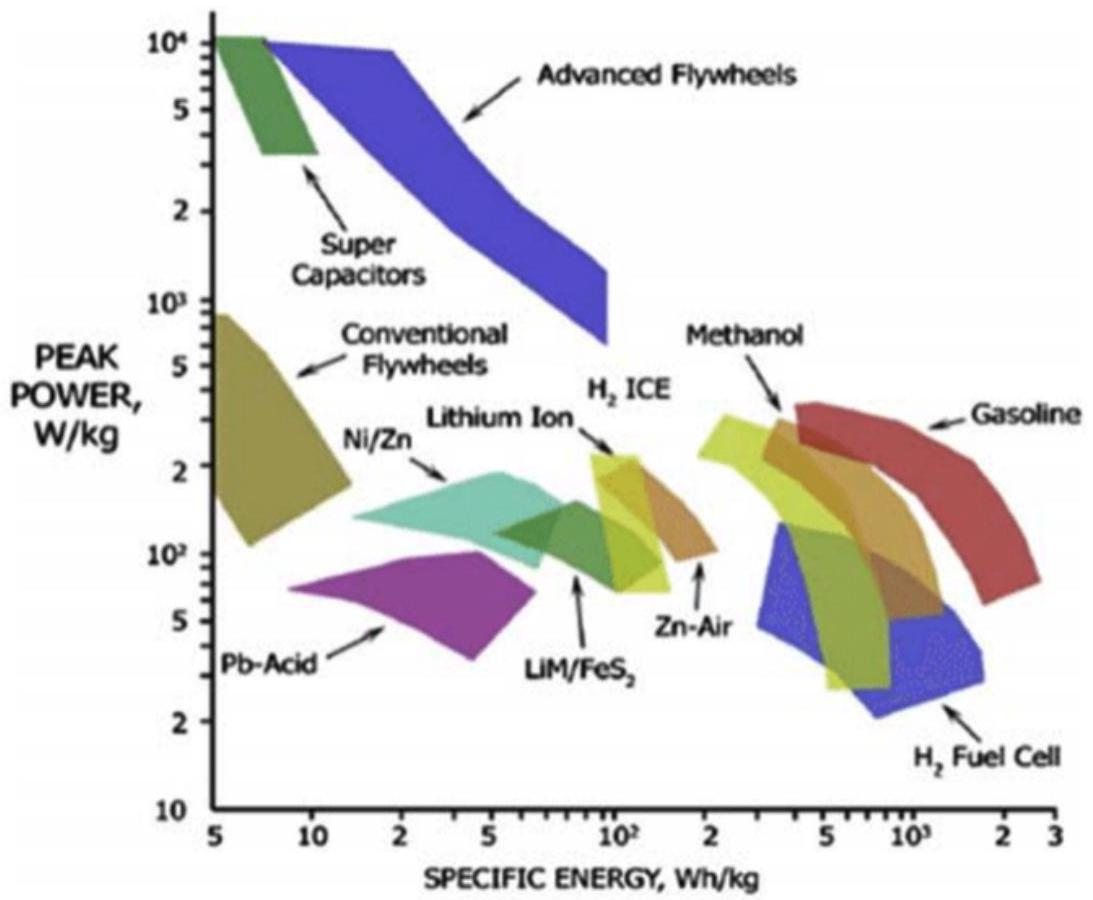
\includegraphics[width=\textwidth]{images/power_vs_energy.jpg}
  \end{column}
  \begin{column}{0.35\textwidth}
    High power/energy ratio required to compensate lack of dynamics for load and generation following.
  \end{column}
\end{columns}

\end{frame}

\begin{frame}{Physical constitution of a battery}
\begin{itemize}
  \item Electrodes: cathode and anode
  \item cathode: from where conventional current (+ charges) leaves -> + electrode if generator.
  \item Electrolyte
  \item Case / enclosure
\end{itemize}

Voltage and current rating are function of material and construction.\\
The surface area of each cell determines factors such as

\begin{itemize}
  \item the total energy stored,
  \item the maximum rates of charge and discharge
\end{itemize}

Example: standard 12 V lead-acid battery: six 2 V cells in series within an enclosure, that is either vented or sealed; the electrolyte can be a liquid or a gel.
\end{frame}


\section{Lead-acid batteries}
\begin{frame}{Composition}

\begin{columns}
  \begin{column}{0.45\textwidth}
    \begin{itemize}
      \item Lead $P b$ (negative electrode)
      \item Lead dioxide $\mathrm{PbO}_{2}$ (positive electrode)
      \item Sulfuric acid $\mathrm{H}_{2} \mathrm{SO}_{4}$ and water in the electrolyte
    \end{itemize}  
  \end{column}
  \begin{column}{0.45\textwidth}
    Chemical reactions in the video below. \\[\baselineskip]
    \href{https://youtu.be/rhIRD5YVNbs}{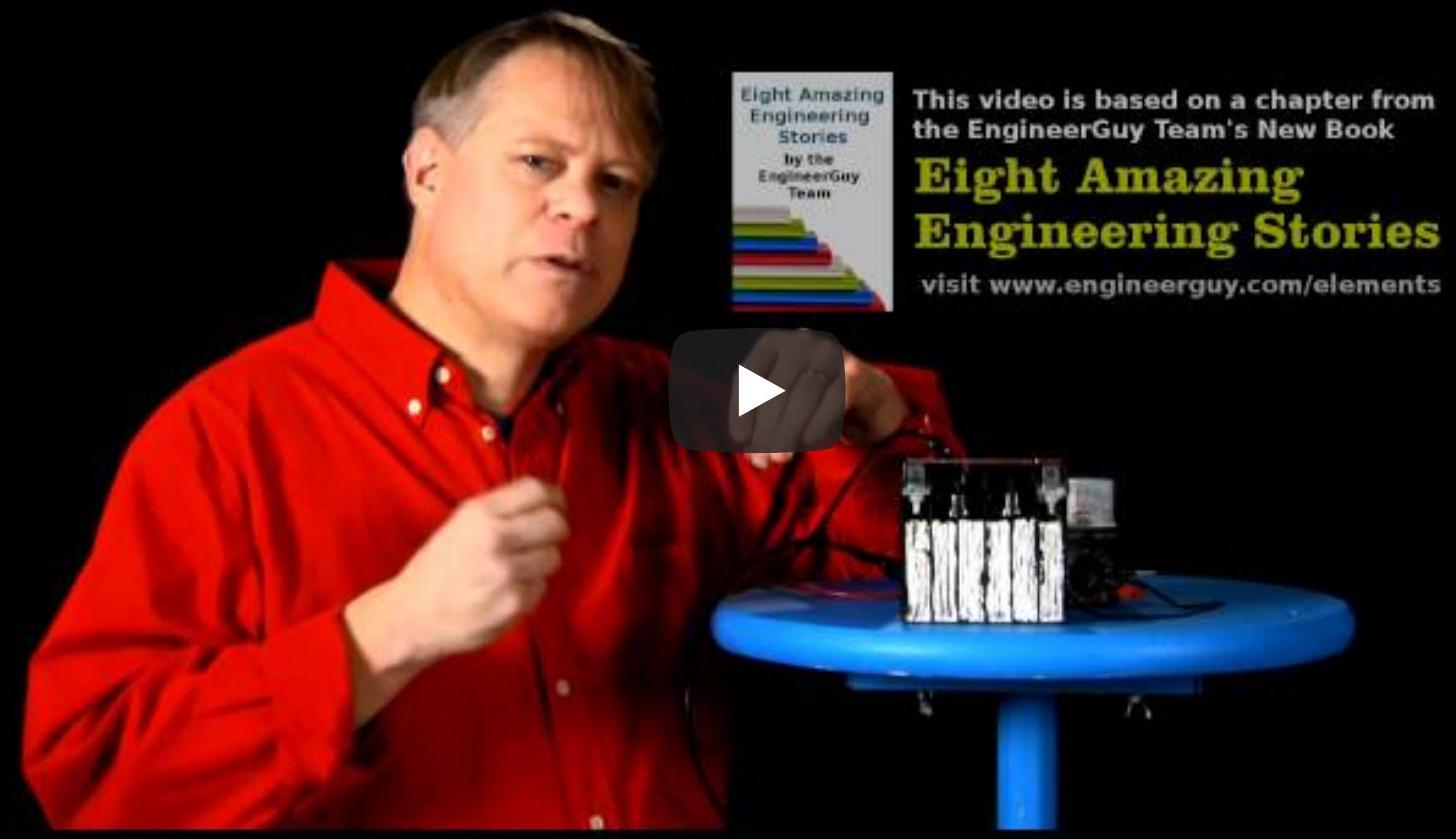
\includegraphics[width=0.95\textwidth]{images/video_Lead_1.jpg}}
  \end{column}
\end{columns}

\end{frame}

\begin{frame}{What limits the cycle-life?}
During discharge, both electrode reactions create PbSo4 (lead sulphate) that coats the electrodes

\begin{itemize}
  \item Lead sulphate is not totally removed when charging
  \item it accumulates with cycles
\end{itemize}

Sulfuric acid concentration dereases (as a consequence of the above phenomenon)

\begin{itemize}
  \item \textbf{flooded} lead-acid batteries can be replenished
  \item \textbf{sealed} lead-acid batteries cannot
\end{itemize}

To avoid accelerating the sulfation process, batteries need to be fully charged after every discharge and they must be kept charged at a float voltage higher than the nominal voltage (2V).

\end{frame}\begin{frame}{Nernst equation recap}
The relationship between battery-stored energy or capacity and electrolyte solution concentration is given by Nernst equation

$$
E=E^{0}+\frac{k T}{q} \ln (Q)
$$

\begin{itemize}
  \item $E^{0}$ is the energy at a standard 1 molar concentration
  \item $k$ is the Boltzmann constant,
  \item $T$ is the temperature in kelvin
  \item $q$ is the charge of an electron.
\end{itemize}

Stored energy is heavily dependent not only on the molar concentration but also on the temperature.

\end{frame}\begin{frame}{Efficiency}
The overal efficiency
$$
\eta=\eta_{V} \eta_{C}
$$

is the product of
\begin{itemize}
  \item a voltage efficiency, ratio of the charge and discharge voltages, and technology dependent (VRLA $=88 \%$ )
  \item a coulombic efficiency, usually $92 \%$
\end{itemize}

\end{frame}\begin{frame}{Efficiency varies with usage}
Battery capacity is indicated in Ah (ampere-hour) (or Wh) for a given discharge rate, which at full capacity is often 8 or 10 hours.

The internal resistance typically varies with different discharge rates, hence the capacity is less if the battery is discharged faster (Peukert’s Effect).

\end{frame}

\begin{frame}[allowframebreaks]{Efficiency and technologies, from Victron's website:}
\begin{enumerate}
  \item \textbf{VRLA technology}: stands for Valve Regulated Lead Acid, which means that the batteries are sealed. Gas will escape through the safety valves only in case of overcharging or cell failure. VRLA batteries are maintenance free for life.
  \item Sealed (VRLA) \textbf{AGM Batteries}: AGM stands for Absorbent Glass Mat. In these batteries the electrolyte is absorbed into a glass-fibre mat between the plates by capillary action. (...) more suitable for short-time delivery of high currents than gel batteries.
  \item Sealed (VRLA) \textbf{Gel Batteries}: the electrolyte is immobilized as gel. Gel batteries in general have a longer service life and better cycle capacity than AGM batteries.
\end{enumerate}


\begin{columns}
  \begin{column}{0.6\textwidth}
    {\footnotesize
  \begin{tabularx}{\textwidth}{rXXXX}
  \toprule
  Discharge time & End Voltage & AGM 'Deep Cycle' & Gel 'Deep Cycle' & Gel 'Long Life' \\
  (constant current) & V & \% & \% & \% \\
  \midrule
  20 hours & 10,8 & 100 & 100 & 112 \\
  10 hours & 10,8 & 92 & 87 & 100 \\
  5 hours & 10,8 & 85 & 80 & 94 \\
  3 hours & 10,8 & 78 & 73 & 79 \\
  1 hour & 9,6 & 65 & 61 & 63 \\
  30 min. & 9,6 & 55 & 51 & 45 \\
  15 min. & 9,6 & 42 & 38 & 29 \\
  10 min. & 9,6 & 38 & 34 & 21 \\
  5 min. & 9,6 & 27 & 24 &  \\
  5 seconds &  & 8 C & 7 C &  \\
  \bottomrule
\end{tabularx}}
  \end{column}
  \begin{column}{0.35\textwidth}
    Effective capacity as a function of discharge time (the lowest row gives the maximum allowable 5 seconds discharge current)
  \end{column}
\end{columns}


\end{frame}

\section{Lithium lon batteries}
\begin{frame}{Lithium lon batteries}
Lithium-ion (Li-ion) batteries have many advantages over lead-acid batteries:

\begin{enumerate}
  \item Lighter than lead-acid batteries because lithium and carbon are lighter than lead.
  \item Do not build up deposits every charge/discharge cycle, so their efficiency is about 99\% -> cycle-life much bigger
  \item Allow deeper discharges (although cycle-life dependes on DoD)
\end{enumerate}

Also, higher cell voltage means fewer series-connected cells for a same string voltage.

\end{frame}

\begin{frame}[allowframebreaks]{Some more explanations}
\begin{center}
  \href{https://youtu.be/VxMM4g2Sk8U}{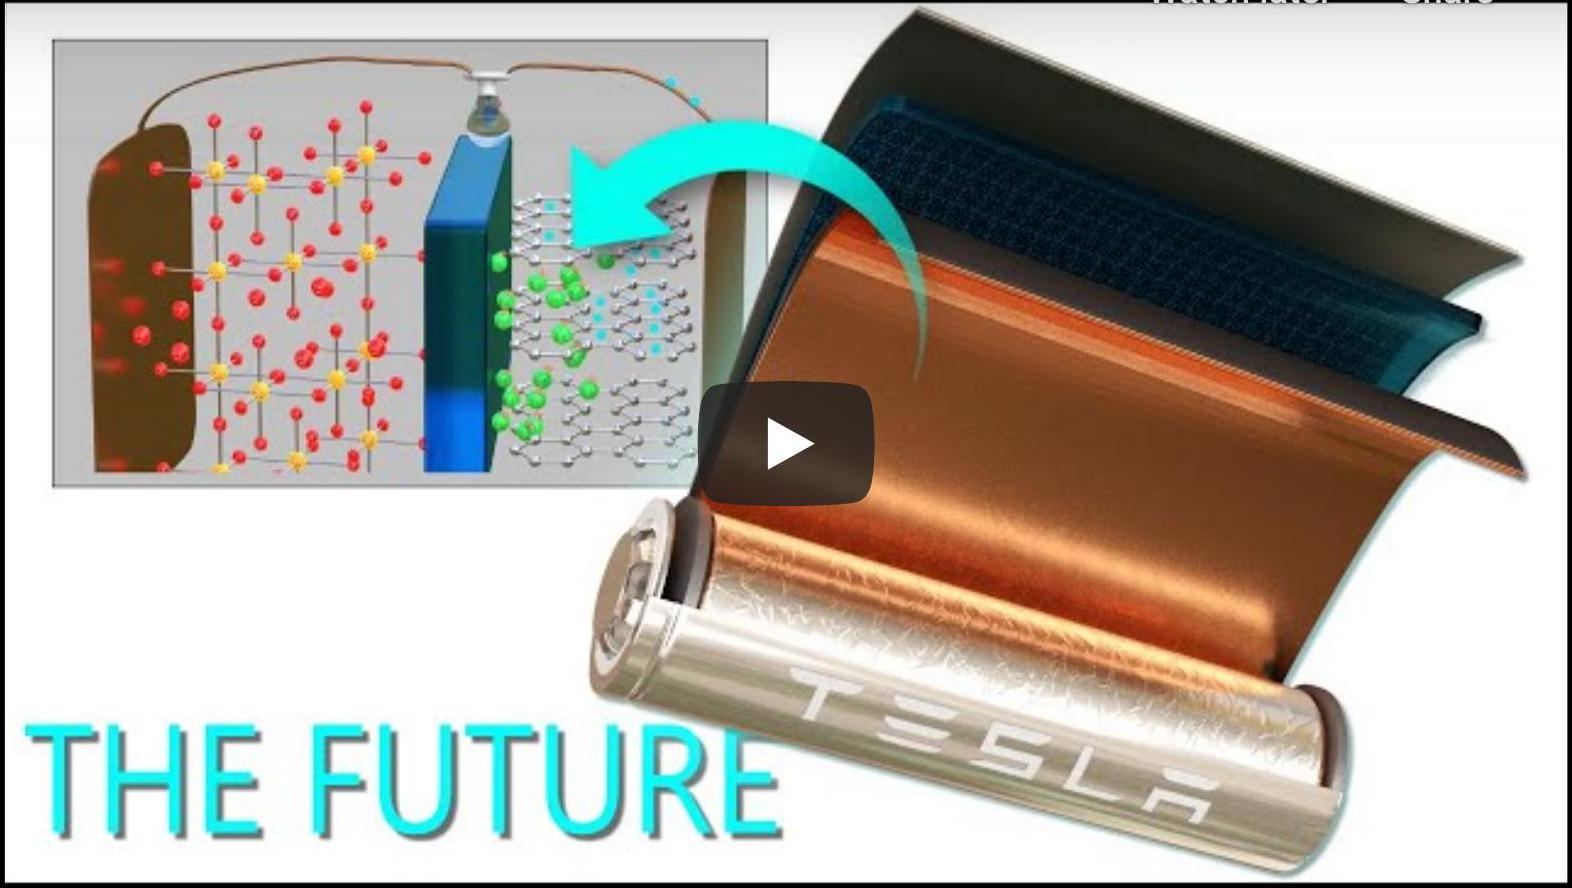
\includegraphics[width=0.6\textwidth]{images/e7c418a7-6530-46e7-9e4a-0de0bdcf74a7-18_888_1572_434_391}}\\
  \href{https://youtu.be/PVnQ87Fvsk4}{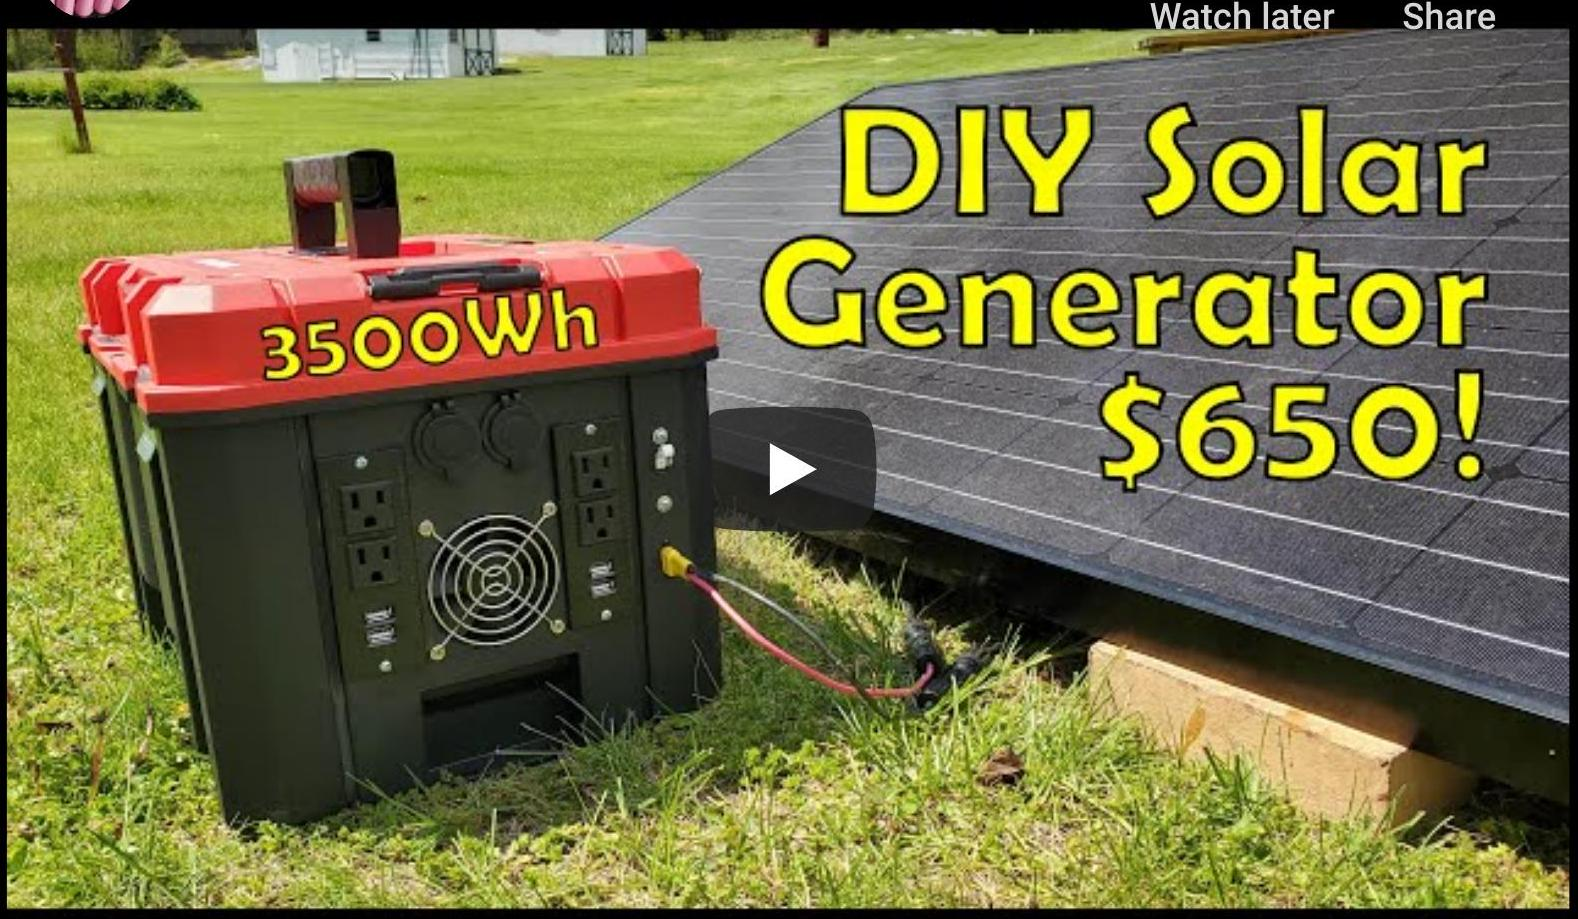
\includegraphics[width=0.6\textwidth]{images/e7c418a7-6530-46e7-9e4a-0de0bdcf74a7-19_919_1578_411_225}}
\end{center}
\end{frame}

\begin{frame}{Battery Management System}
\begin{itemize}
  \item Modern battery storage systems are equipped with a battery management system (BMS).
  \item The BMS serves two main purposes:
  \begin{itemize}
    \item Monitoring: harvest data to be fed to control systems and graphical user interface.
    \item Safety: ensure battery does not operate in dangerous regimes, e.g. severe overvoltage or high temperature. Cell balancing.
  \end{itemize}
  \item Old BMSs used inaccurate heuristics to estimate operating parameters and stop operation if needed whereas new generations exploit - high-fidelity electrochemical models solved in real-time.
\end{itemize}

\end{frame}\begin{frame}{Comparison of Li-lon Battery Technologies}
\begin{center}
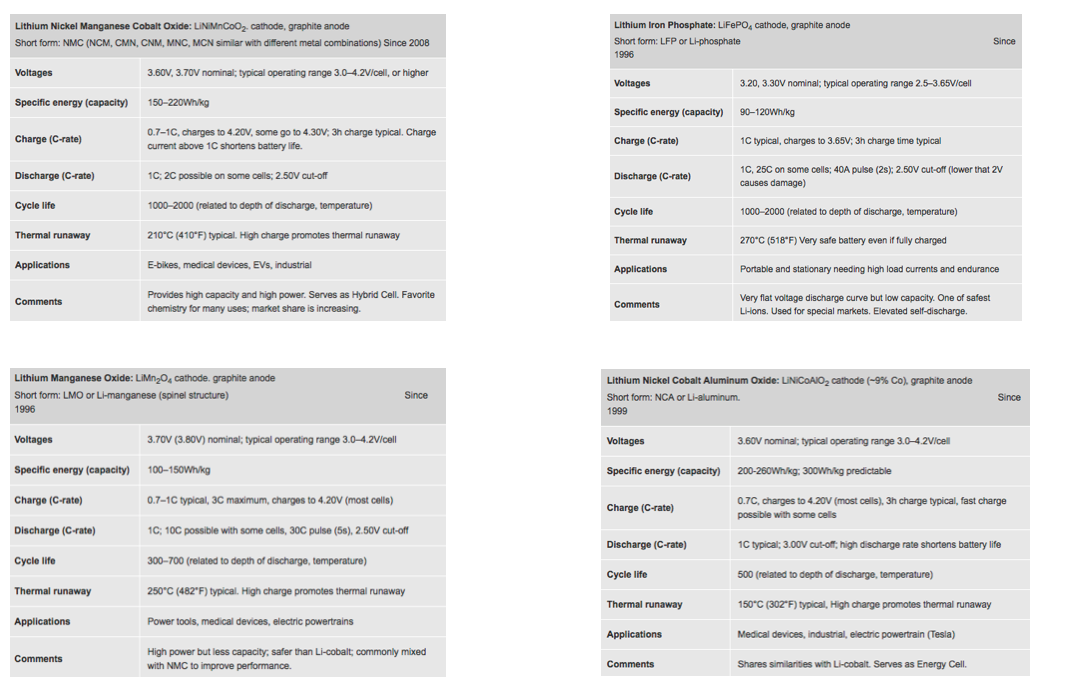
\includegraphics[width=0.7\textwidth]{images/comparison_Li.png}
\end{center}
\end{frame}

\section{Flow batteries}
\begin{frame}[allowframebreaks]{Flow batteries}
\begin{center}
  \href{https://youtu.be/AagO07cHRG8}{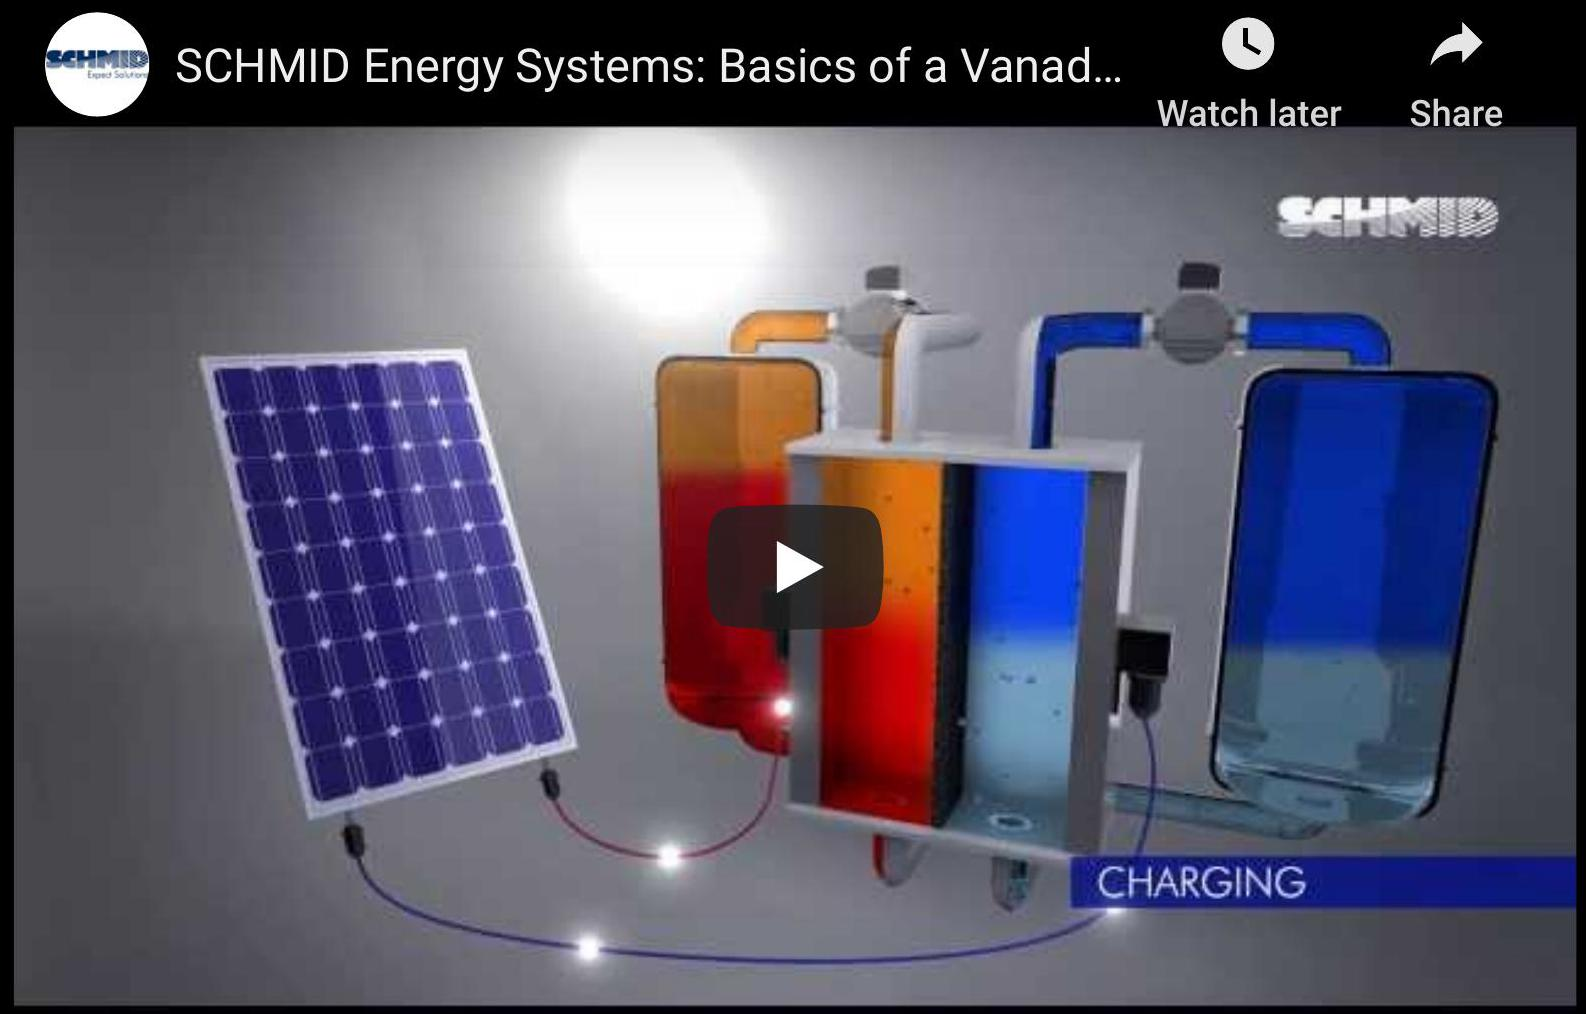
\includegraphics[width=0.6\textwidth]{images/e7c418a7-6530-46e7-9e4a-0de0bdcf74a7-24_1014_1586_222_382}}
\end{center}

\begin{center}
  \href{https://youtu.be/UT8vjThfWB4}{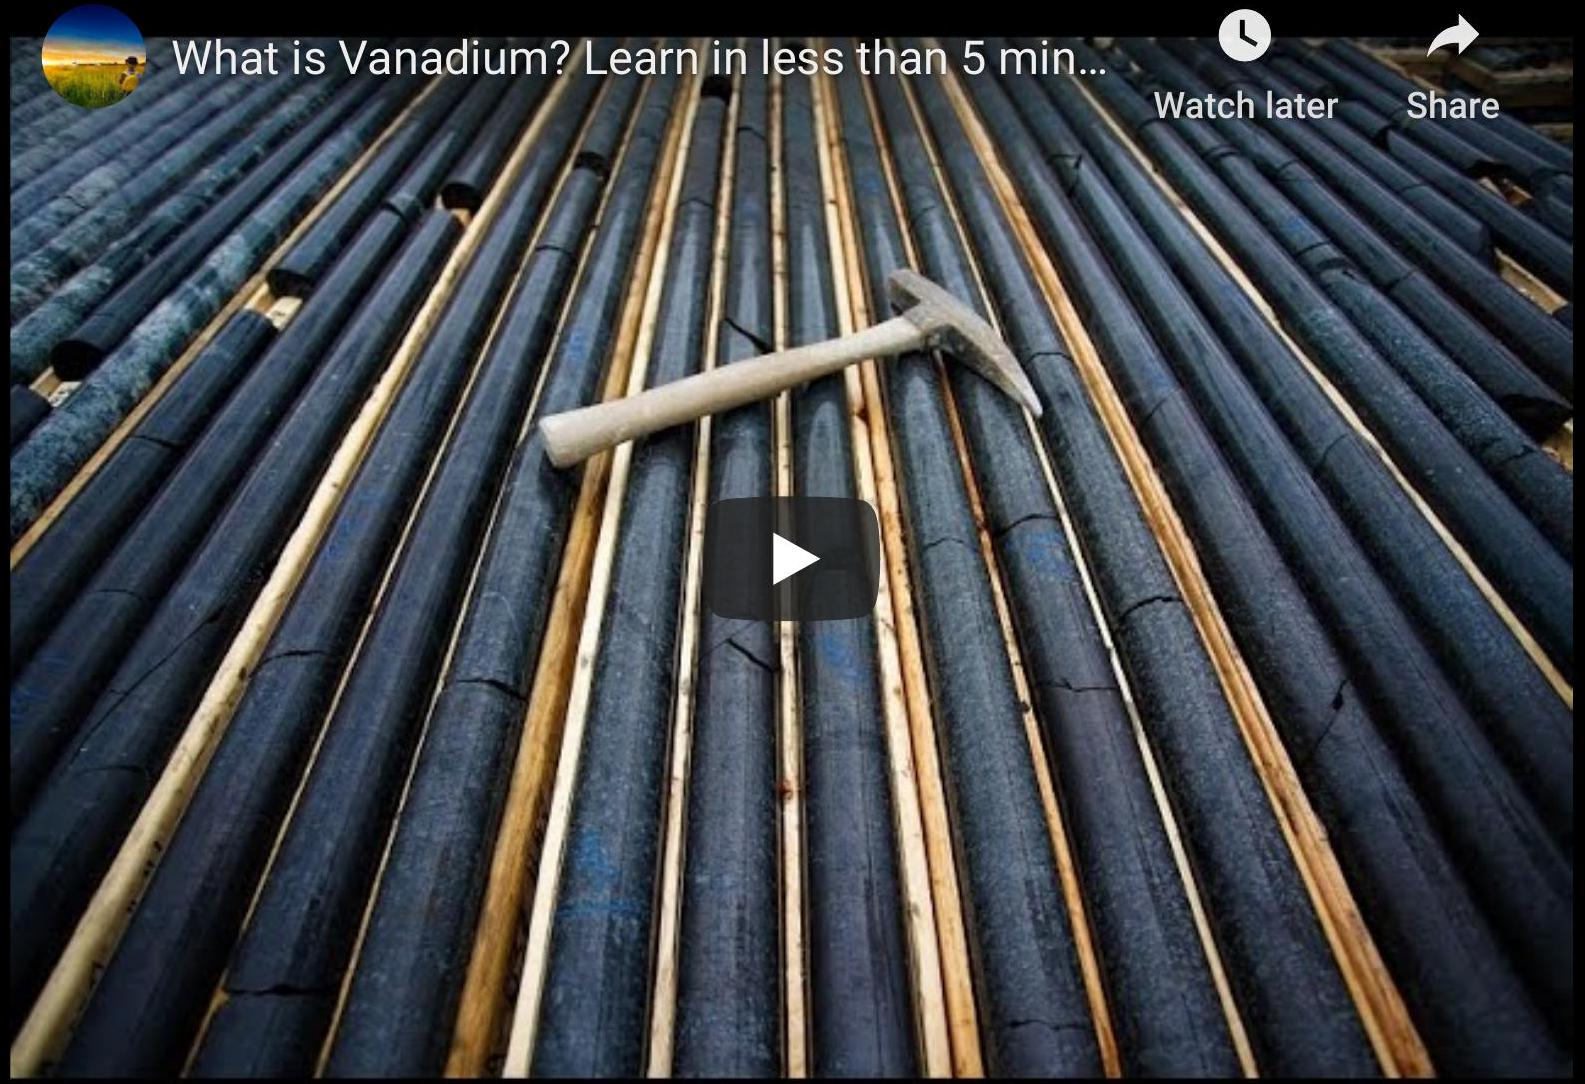
\includegraphics[width=0.6\textwidth]{images/e7c418a7-6530-46e7-9e4a-0de0bdcf74a7-25_1084_1585_285_289}}
\end{center}
\end{frame}

\section{Essential Battery Parameters}
\begin{frame}{Capacity, SOC \& Voltage}

\begin{columns}
  \begin{column}{0.45\textwidth}
    \begin{itemize}
      \item \textbf{Capacity} reflects total amount of charge (Ah) that can be theoretically stored in device.
      \item \textbf{State of charge (SOC)} reflects amount of charge available at given time instant, usually expressed as percentage of capacity.
      \item \textbf{Voltage (V)} at cell/pack terminals is measurable operating parameter providing indirect information about SOC.
    \end{itemize}
  \end{column}
  \begin{column}{0.45\textwidth}
    \begin{center}
      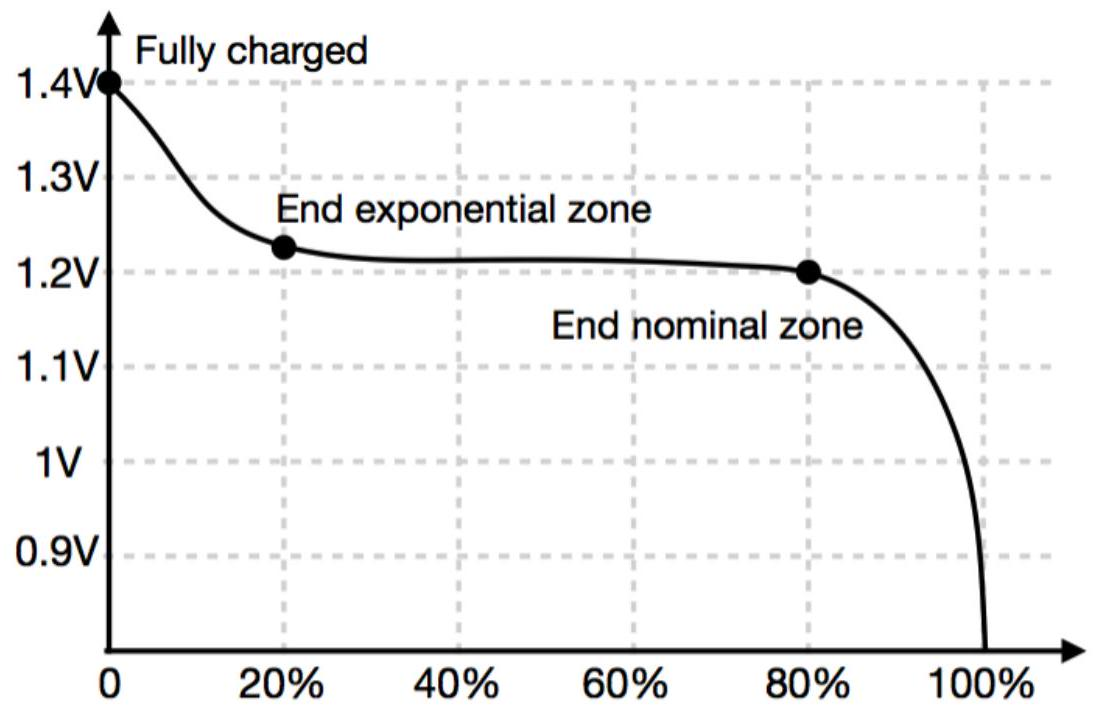
\includegraphics[width=\textwidth]{images/e7c418a7-6530-46e7-9e4a-0de0bdcf74a7-28_713_1097_768_628}\\
    {Figure 2.2: Discharge curve example.}
    \end{center}
  \end{column}
\end{columns}
\end{frame}

\begin{frame}{Current \& C-rate}
\begin{itemize}
  \item \textbf{Current (A)} is the main excitation signal in batteries as voltage is imposed by system physics.
  \item \textbf{C-rate} is a standardized metric quantifying applied current intensity. This alternative scale is derived from the constant current intensity needed to fully charge/discharge the battery over a given time period, usually 1 h .
  \item Battery charge/discharge behaviors vastly differ across C-rate range.
  \item In particular, in Li-ion cells, much less charge can be retrieved from discharge at high C-rates. This phenomenon is called the rate - capacity effect.
\end{itemize}

\end{frame}\begin{frame}{Degradation \& Health}
\begin{itemize}
  \item Battery performances typically decrease over lifetime, in a process known as degradation.
  \item Main degradation types:
  \begin{itemize}    
    \item \textbf{Power fade}: peak power decreases over time.
    \item \textbf{Capacity fade}: capacity decreases over time.
  \end{itemize}
  \item Several metrics quantifying degradation exist, e.g. remaining capacity or internal resistance. Those quantities then allow to define state of health indicator in fashion similar to SOC.
\end{itemize}

\end{frame}\begin{frame}{Battery models in practice}

Highly dependent of the application :
\begin{itemize}
  \item for sizing or planning problems, a simple tank model may be enough (for sizing, see how to evaluate capacity degradation on the next slide)
  \item a more detailed model can represent the current-voltage dependance and thus the efficiency as a function of the power charged or discharged:\\
\end{itemize}
\begin{columns}
  \begin{column}{0.3\textwidth}
    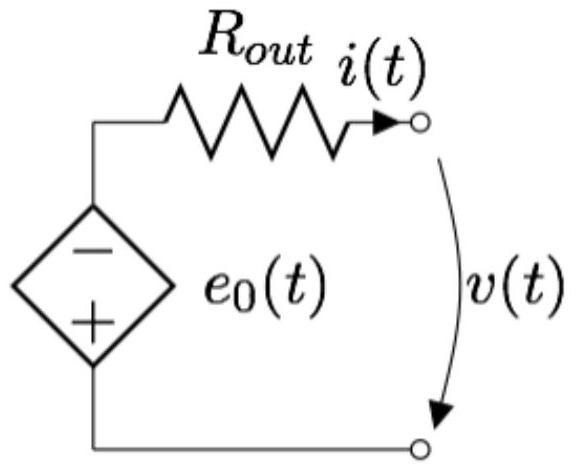
\includegraphics[width=\textwidth]{images/e7c418a7-6530-46e7-9e4a-0de0bdcf74a7-31_468_576_711_444}
  \end{column}
  \begin{column}{0.55\textwidth}
    Parameters can be obtained from a data sheet, or from voltage [dis]charge curves experiments
  \end{column}
\end{columns}
\end{frame}


\begin{frame}{Simple model of energy capacity degradation as a function of the number of cycles}

For Li-ion batteries, a simple throughput model is in general enough to evaluate the number of cycles:\\

\begin{itemize}
  \item cycles(t) = amount of Ah charged(t) / initial\_capacity\\
  \item Actual capacity $(\mathrm{t})=$ initial capacity $-a^{*} \operatorname{cycles}(\mathrm{t})$\\
\end{itemize}
$a$ is a parameter determined experimentally.
\end{frame}

\begin{frame}{Charging strategies}

Charging strategies refer to the way current and voltage are controled over time to charge a battery.

Complex strategies exist to maximize the efficiency and the safety of the process

\begin{itemize}
  \item constant current CC is the simplest, but can lead to over voltage if not stopped fast enough
  \item constant voltage CV is a bit more complex, but avoids over-voltages (since it is regulated). But leads to high currents when the battery is near empty and tiny currents when it is almost charged.
  \item more advanced techniques combining CC and CV or regulating a function of C and improve the process.
\end{itemize}

\end{frame}\begin{frame}{State of charge estimation}
\begin{itemize}
  \item Coulomb counting
  \item Voltage measurment
  \item Kalman filtering
  \item Technology specific methods.
\end{itemize}
\end{frame}

\section{Capacitors and supercapacitors}
\begin{frame}{Capacitors}
\begin{itemize}
  \item Energy stored in electrostatic form (electrical field).
  \item Charge (electrons) stored on electrode surfaces.
  \item Dielectric inserted between electrodes to increase capacity.
  \item Two common designs: ceramic/film capacitors and electrolytic capacitors (with much higher capacity).
\end{itemize}

\end{frame}

\begin{frame}{Schematic of common capacitor technologies}
\begin{center}
  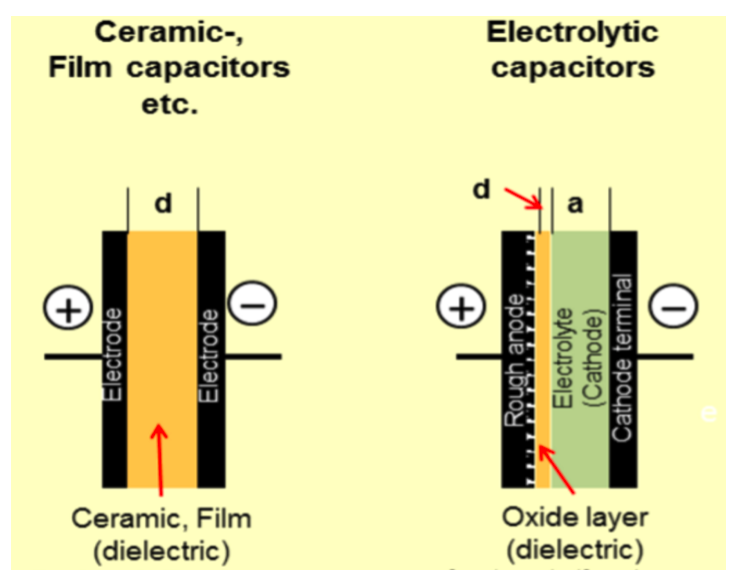
\includegraphics[width=0.6\textwidth]{images/capacitor.png}
\end{center}
\end{frame}

\begin{frame}{Supercapacitors}
\begin{itemize}
  \item Super and ultra capacitors are synonyms. Capacitors and super capacitors are different.
  \item Energy stored in electrostatic form (electrical field).
  \item Charge (ions) adsorbed on porous activated carbon electrode surfaces bound to current collector.
  \item Ions transferred through electrolyte from one electrode to the other.
  \item Porous separator inserted between electrodes.
\end{itemize}

\end{frame}\begin{frame}{\Large Schematic \& working principle of super capacitor technology}
\begin{center}
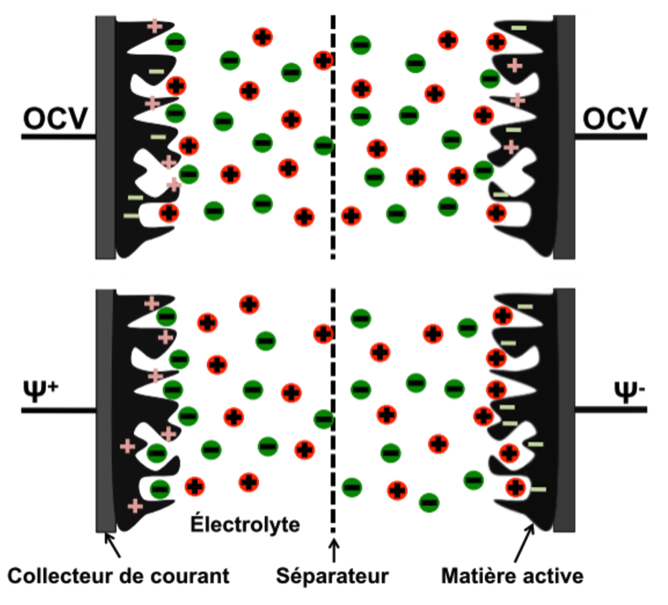
\includegraphics[width=0.5\textwidth]{images/supercapacitor.png}
\end{center}
\end{frame}

\begin{frame}{E.g. Maxwell ultracapacitors}
  \centering
%Optimized for size and power in industrial, electronics, and consumer applications\\
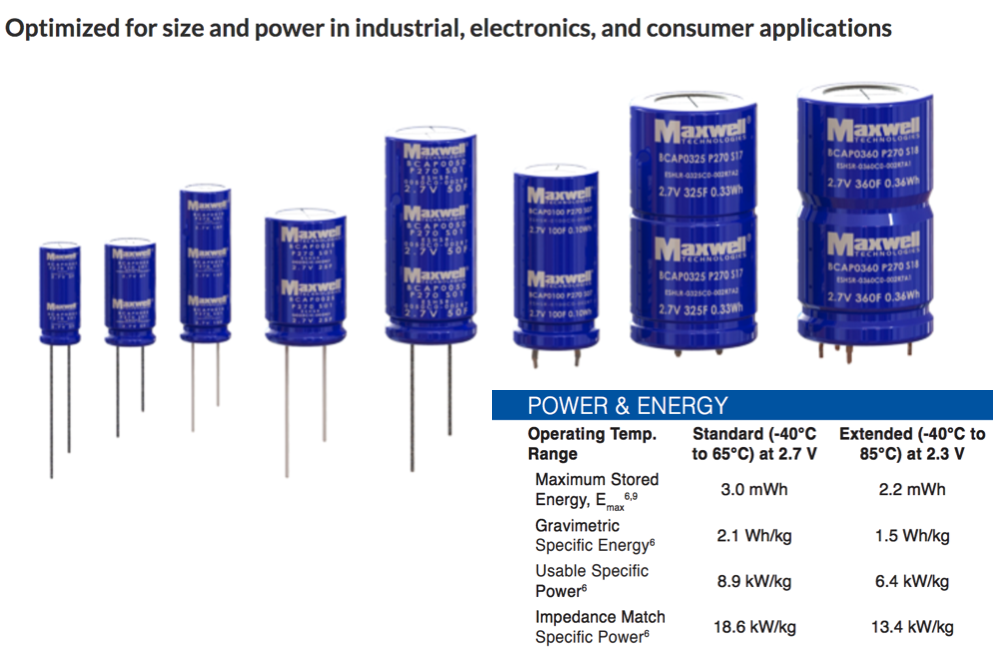
\includegraphics[width=0.7\textwidth]{images/maxwell_supercaps.png}
\end{frame}

\begin{frame}{Size comparison}

  \begin{columns}
  \begin{column}{0.45\textwidth}
  \begin{center}
    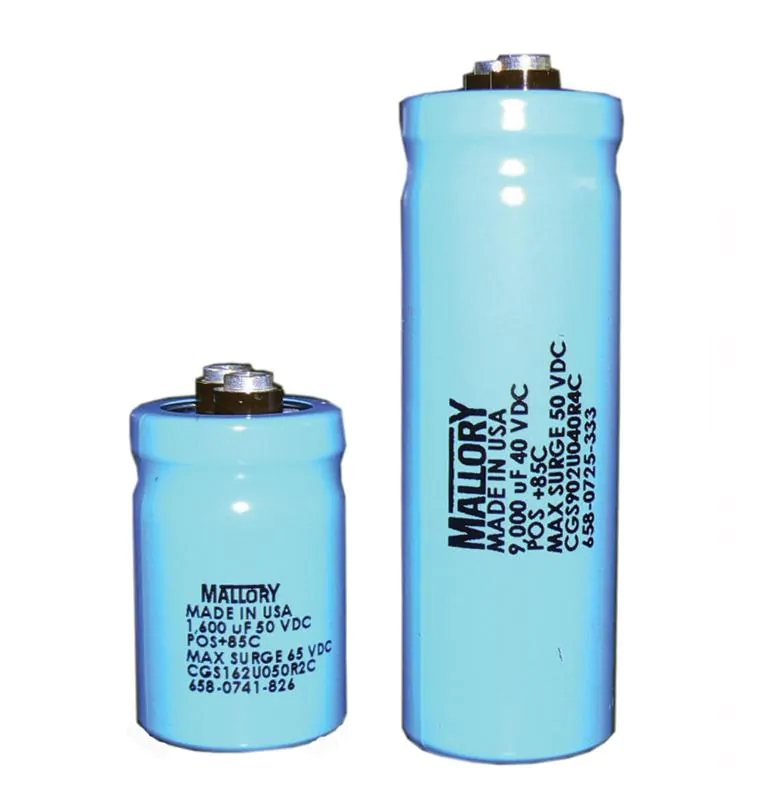
\includegraphics[width=0.6\textwidth]{images/real_capacitor.png}
    \end{center}

    Capacitor of 1F: cylinder with

    \begin{itemize}
      \item diameter $=7.6 \mathrm{~cm}$
      \item length $=14.3 \mathrm{~cm}$
    \end{itemize}
  \end{column}
  \begin{column}{0.45\textwidth}
    \begin{center}
    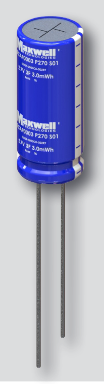
\includegraphics[width=0.05\textwidth]{images/real_ultracap.png}
    \end{center}

    Capacitor of \alert{3F}: cylinder with

    \begin{itemize}
      \item diameter $=0.8 \mathrm{~cm}$
      \item length $=2 \mathrm{~cm}$
    \end{itemize}
  \end{column}
\end{columns}
\end{frame}